% -*- latex -*-
%-----------------------------------------------------------------------
%;  Copyright (C) 2002
%;  Associated Universities, Inc. Washington DC, USA.
%;
%;  This program is free software; you can redistribute it and/or
%;  modify it under the terms of the GNU General Public License as
%;  published by the Free Software Foundation; either version 2 of
%;  the License, or (at your option) any later version.
%;
%;  This program is distributed in the hope that it will be useful,
%;  but WITHOUT ANY WARRANTY; without even the implied warranty of
%;  MERCHANTABILITY or FITNESS FOR A PARTICULAR PURPOSE.  See the
%;  GNU General Public License for more details.
%;
%;  You should have received a copy of the GNU General Public
%;  License along with this program; if not, write to the Free
%;  Software Foundation, Inc., 675 Massachusetts Ave, Cambridge,
%;  MA 02139, USA.
%;
%;  Correspondence concerning AIPS should be addressed as follows:
%;          Internet email: aipsmail@nrao.edu.
%;          Postal address: AIPS Project Office
%;                          National Radio Astronomy Observatory
%;                          520 Edgemont Road
%;                          Charlottesville, VA 22903-2475 USA
%-----------------------------------------------------------------------
%Body of intermediate AIPSletter for 31 December 2001

\documentclass[twoside]{article}
\usepackage{graphics}

\newcommand{\AIPRELEASE}{December 31, 2002}
\newcommand{\AIPVOLUME}{Volume XXII}
\newcommand{\AIPNUMBER}{Number 2}
\newcommand{\RELEASENAME}{{\tt 31DEC02}}
\newcommand{\OLDNAME}{{\tt 31DEC01}}

%macros and title page format for the \AIPS\ letter.
\input LET98.MAC
%\input psfig

\newcommand{\MYSpace}{-11pt}

\normalstyle

\section{General developments in \AIPS}

\subsection{Linux news: bad compilers}

Instructions for fetching and installing the GNU 2.95.3 compiler are
given on the \AIPS\ web page.  The tar file is directly available from
NRAO\@.  This is needed since the 2.96.x compiler does not optimize
code properly and the newer GNU 3.0 through 3.2 versions of g77
produce code that executes up to 20\%\ slower than that produced by
the older version.

\subsection{Current and future releases}

We now have formal \AIPS\ releases on an annual basis with binary
releases only for Solaris and Linux.  All architectures can do a full
installation from the source files.  The current release is called
{\tt 31DEC02} and is now frozen.  If you took a development copy of
this version at some earlier date, you may use the ``Midnight Job''
(MNJ) to bring it up to date.  You need to run a MNJ only once in 2003
to convert your copy of {\tt 31DEC02} into the now frozen version.
This \Aipsletter\ is intended to advise you of developments in this
release.

We have begun a new version, called {\tt 31DEC03}, which is now under
development by the (reduced) \AIPS\ Group.  You may fetch and install
a complete copy of this version at any time.  Having fetched {\tt
31DEC03}, you may update your installation whenever you want by
running the MNJ which uses transaction files to copy and compile the
code selectively based on the code changes and compilations we have
done.  We expect users to take the source-only version of {\tt
31DEC03} \AIPS\ over the Internet (via \emph{anonymous} ftp).

The MNJ has been changed.  The secure shell, with all its fragile
complexities, is no longer required.  Instead {\tt mnj.aoc.nrao.edu}
will serve up \AIPS\ incrementally --- or as a whole --- using the
Unix tool {\tt cvs} running with anonymous ftp.  Linux sites will
almost certainly have {\tt cvs} installed; other sites may have
installed it along with other GNU tools.  Secondary MNJs will still be
possible using {\tt ssh} or {\tt rcp} or NFS as with previous
releases.  We have found that {\tt cvs} works very well, although it
has one quirk.  If a site modifies a file locally but in an
\AIPS-standard directory, {\tt cvs} will detect the modification and
attempt to reconcile the local version with the NRAO-supplied version.
This usually produces a file that will not compile or run as
intended.

\AIPS\ is now copyright \copyright\ 1995 through 2003 by Associated
Universities, Inc., NRAO's parent corporation, but may be made freely
available under the terms of the Free Software Foundation's General
Public License (GPL)\@.  This means that User Agreements are no longer
required, that \AIPS\ may be obtained via anonymous ftp without
contacting NRAO, and that the software may be redistributed (and/or
modified), under certain conditions.  The full text of the GPL can be
found in the \texttt{15JUL95} \Aipsletter.

\subsection{Installing a new version}

Some managers of sites that run only the current development version
of \AIPS\ have asked whether they could upgrade {\tt 31DEC02} to {\tt
31DEC03} by a simple renaming of the directories and editing of the
{\tt AIPSPATH} files.  We have tried this and it did not work.  There
are a bunch of link files that have to be redone and even then, {\tt
cvs} is too smart and fetches {\tt 31DEC02} control files.  It might
be possible to revise even more files to override this behavior, but
at this level it becomes simpler, quicker, and very much more reliable
simply to install {\tt 31DEC03} from the {\tt tar} ball.

When installing a new \AIPS\ release in a system that already has a
previous release, we recommend that {\tt install.pl} be used and that
the previous release be left in place, at least until the installation
has been seen to work.  If you do this, then you will not have to
re-edit the disk, printer, and tape lists and can simply skip all
those pages in the {\tt install.pl} menus.  The old {\tt
\$HOME/.AIPSRC} file may be left in place, but it will need to be
edited.  The lines giving the {\tt DOWNLOADED} and {\tt UNPACKED}
parameters should be deleted and the {\tt CCOMOPT} line should be
changed to point to the current release rather than the previous one
--- the {\tt -I} parameter really should be {\tt -I\$INC} but that
seems to confuse {\tt install.pl}.  Therefore, for now, the {\tt
\$INC} has to be given in its full path name, which forces a re-edit
with each release.  If you have made special versions of {\tt
UPDCONFIG} and {\tt do\_daily.{\it host}}, you should preserve them
under new names and restore them after the install.  The {\tt
\$AIPS\_ROOT/AIPSPATH.*SH} files will need to be edited after the
install  if you wish to run multiple different versions of \AIPS\@.

For Linux and Solaris Ultra systems only, a binary installation is
available from CDrom, supported by {\tt install.pl}.  Alternatively,
there are binary files which may be downloaded from\\
\centerline{{\tt
ftp://ftp.aoc.nrao.edu/pub/software/aips/31DEC02}.}\\
With a modern computer, it will probably be faster to recompile the
programs locally using {\tt install.pl}.

\section{Patch Distribution for {\tt 31DEC01}}

As before, important bug fixes and selected improvements in
\OLDNAME\ can be downloaded via the Web beginning at:

\begin{center}
\vskip -10pt
{\tt http://www.aoc.nrao.edu/aips/patch.html}
\vskip -10pt
\end{center}

Alternatively one can use {\it anonymous} \ftp\ on the NRAO CPU {\tt
aips.nrao.edu}.  Documentation about patches to a release is placed
in the anonymous-ftp area {\tt pub/aips/}{\it release-name} and the
code is placed in suitable subdirectories below this.   Information on
patches and how to fetch and apply them is also available through the
World-Wide Web pages for \AIPS\@.  As bugs in {\tt 31DEC03} are found,
they are simply corrected since {\tt 31DEC03} remains under
development.  Corrections and additions are made with a midnight job
rather than with manual patches.  Remember, no matter when you
received your copy of \OLDNAME\ or {\tt 31DEC02} {\it you must} fetch
and install its patches if you require them.

The \OLDNAME\ release had a few important patches including a new one
in September.  These were:
\begin{enumerate}
\item\ {\tt SAD}, {\tt JMFIT}, and {\tt IMFIT} fail to handle the
      primary beam correction properly for offset fields {\it
      2002-02-11}.
\item\ {\tt IMAGR} failed to apply the {\tt IMAGRPRM(11)} parameter to
      the peak in the Clean windows {\it 2002-02-19}.
\item\ {\tt SPLAT} failed to average spectral channels properly for
      multiple IFs {\it 2002-06-20}.
\item\ {\tt BPASS} failed to include the first record of each {\tt
      SOLINT} {\it 2002-09-16}.
\end{enumerate}
\vfill\eject

\section{Improvements of interest to users in \RELEASENAME}

We expect to continue publishing the  \Aipsletter\ approximately every
six months along with the annual releases.  Despite the reduction in
personnel, there have been a number of changes in {\tt 31DEC02}.  In
the last edition, we reported on three new tasks: {\tt WETHR} to plot
the contents of the weather table including flagging data based on the
contents of the table, {\tt BOXES} to add Clean boxes to a {\tt
BOXFILE} based on source catalogs, and {\tt UVDEC} to copy a \uv\ data
set retaining only every $n^{\uth}$ spectral channel.  There were also
three new verbs: {\tt TKERASE} to clear the contents of the Tektronix
emulation display window, {\tt SG2RUN} to convert the contents of a
{\tt SAVE}/{\tt GET} file into a {\tt RUN} file for use on another
computer and/or user number, and {\tt OUTPUTS} to show those adverbs
whose values will be changed when running the task.  A new {\tt RUN}
file called {\tt WRTPROCS} provides three procedures for automated
writing and reading of FITS disk files.

In the last six months, we have developed two new tasks: {\tt WIPER}
to edit \uv\ data interactively from a {\tt UVPLT}-like display and
{\tt LOCIT} to solve for antenna positions.  For the VLA, the latter
replaces an ad hoc pair of programs that only ran on Solaris and were
no longer maintainable.  The VLBA pipeline reduction {\tt VLBAPIPE}
package has been publicly released.  ``Color'' was added to \AIPS'
plotting.  This allows contrasting symbols and contour and
polarization lines to be drawn on top of gray-scales.  Full pseudo-
and true-coloring were also made available.  A wide variety of tasks
were enhanced in some way.

Other than relatively minor differences, {\tt 31DEC02} is compatible
in all major ways with the 2001, 2000, 1999, and {\tt 15OCT98}
releases.  There are significant incompatibilities with older
versions.

\subsection{Plotting in color}

Several new plot command codes have been developed: line type
(values 1--4), dark vector, write RGB gray-scale, initialize for
color gray-scales, and write bright and dark characters inside plot
area.  These allow different line types to be assigned different
colors both when they are bright or when they need to be ``dark''
because they are drawn over significant gray-scale brightness.  They
allow the labeling, contouring, polarization vector drawing, and
``star'' plotting routines to draw in a contrasting color when the
background gray-scale is strong.  They allow the conversion of
gray-scales with a color table (called an ``output-function-memory''
or ``OFM'') to pseudo colors and the full display of a true-color
(RGB) image such as those produced by {\tt TVHUI} and {\tt RGBMP}\@.
Examples of color plotting are given at the end of this \Aipsletter.

All plot tasks in \AIPS\ were changed to use the line-type command.
{\tt GREYS} was changed to support {\tt FUNCTYPE}, to do dark vectors
when needed to plot contours and stars, to read an OFM to color the
gray-scale image, and to construct and display RGB images from an
input RGB image or 3 different input images.  {\tt PCNTR} was changed
to plot gray-scales optionally including {\tt FUNCTYPE}, OFM coloring,
true RGB image display, and dark vectors in the contours, polarization
vectors and stars.  {\tt KNTR} was also changed to plot polarization
vectors and to do the full range of gray-scale plotting including all
the dark vectors and true- and pseudo-color displays.

The task that makes RGB images from images used as images of
intensity, hue, and (optionally) saturation is called {\tt TVHUI}\@.
It was revised to handle axis increments correctly and to offer the
{\tt SQ} transfer function.  {\tt RGBMP} makes RGB cubes by weighted
summing of image planes along the $Z$ axis.  It had an addressing error
that caused it to weight the red and blue images unequally and it
previously ignored the actual direction of the $Z$ axis coordinate so
that red and blue had nothing to do with red-shifted and blue-shifted.
Those bugs were corrected and a number of experimental methods for
doing the summing were added.

The plot rendering tasks {\tt TKPL} and {\tt TXPL} were revised to do
what little they can do with the new commands.  {\tt TVPL} was changed
to implement most of the new commands, giving the user the choice of
rendering all dark vectors as black or leaving them bright.  Since it
puts them in colored graphics overlay planes, they may not require the
use of black.  {\tt TVPL} and all plot tasks with {\tt DOTV = TRUE}
were revised to use either a single graphics overlay for all lines and
characters or to use graphics overlays 1 through 4 for the four
different line types.  The usage of line types varies by plot task.
As a general rule, type 1 is labeling, type 2 is contours, type 3 is
vector drawings such as polarization vectors, and type 4 is for
symbols such as stars or visibility samples.  {\tt LWPLA} is the main
task for converting plot files to paper, transparencies, and journals.
The scaling options for gray-scales were retained, but they will
normally not be needed since it is more natural to apply them in the
plot tasks.  Pseudo-coloring of gray scales was added to {\tt
LWPLA} as was the new adverb {\tt DOCOLOR}\@. If it is true, then the
new adverb array {\tt PLCOLORS(3,10)} is used to color the 4 line
types in bright vectors, the 4 line types in dark vectors, the
characters drawn outside of the main plot, and the background of the
full plot, respectively.  Some journals prefer the ``CMYK'' color
representation used in printing to the usual RGB scheme.  {\tt LWPLA}
now offers the option to use CMYK rather than RGB, but RGB remains the
default since it uses less disk.  The positioning of vertical strings
by {\tt LWPLA} was corrected.

All plot tasks had subtle changes made to the spacing of labels and
plot borders.  {\tt POSSM} was corrected for residual errors related
to plotting multiple IFs and polarizations in a single panel.  It was
made better at actually stopping when done and at honoring {\tt
NPLOTS}\@.  {\tt PROFL} was corrected to choose its plot scaling in a
way more likely to fill the page and to be less sensitive to certain
inevitable plotting errors.  {\tt UVPLT} was given the option to plot
both individual samples and binned averages and the {\tt DOWEIGHT}
adverb was added to control the averaging.  {\tt TVCPS} was changed to
handle very large images when read from disk.

\subsection{UV data handling and calibration}

\subsubsection{WIPER}

{\tt WIPER} is a new task to wipe out (flag) bad data using a {\tt
UVPLT}-like display of the data.  A circular eraser of user-controlled
diameter is used to erase samples from the plot --- or to restore
previously erased samples.  During the interactive phase of the
operation, the samples cannot be identified individually, but their
coordinates in the two axes of the display are shown.  When the
interactive session is terminated, a new flag table is created
containing all previous flags plus the new, potentially numerous,
flags generated by {\tt WIPER}\@.

\subsubsection{LOCIT}

{\tt LOCIT} is a new task to solve for antenna locations from an {\tt
SN} table.  It works best if a series of observations of calibrators
is made with a wide variety of elevations and hour angles.  {\tt
CALIB} then finds the {\tt SN} table for this sequence of scans.  {\tt
LOCIT} works by assuming that the phase of each IF is relatively
stable and that the phases are mostly due to antenna location errors.
Plots and printer displays of the residuals and solutions are
available.  A new {\tt RUN} file called {\tt BASFIT} sets ``normal''
adverb values for a sequence of {\tt CALIB}, {\tt LOCIT}, and {\tt
LWPLA} to be used primarily by the VLA analysts.  {\tt LOCIT} is based
on older programs written by Rick Perley and Gustaaf van Moorsel but
offers greater maintainability and several new options.

\subsubsection{VLA archive data}

The archive of raw VLA data is being placed on-line by the {\tt e2e}
project at the NRAO\@.  The information to select which data you need
is available from NRAO's web site and methods to select all data from
a specific project are being developed.  From the \AIPS\ perspective,
this development made it desirable to read archive data from disk as
well as tape.  {\tt PRTTP} and {\tt FILLM} have both been revised to
read one or more data files from a user-specified disk directory.  The
file names must all be the same except for an appended ``tape-file''
number.

A number of generally minor errors in {\tt FILLM} were corrected while
the disk reading was being tested.  The most serious was in the
handling of ends of file, which could cause the task to get the wrong
file number and to fail to stop as requested.  Odd conditions on-line
could cause {\tt FILLM} to write fewer channel-0 samples than spectral
samples, which was confusing to users.  The data in such cases was
always bad.  History writing was improved as well.

\subsubsection{Other changes}

\begin{description}
\myitem{FITLD} failed to apply the General Relativity correction to
               source coordinates, giving small errors in the apparent
               coordinates.
\myitem{QUACK} was given the option ``{\tt TAIL}'' to flag all sources
               for a specified time following a scan.  This covers the
               case in which the array thinks it has moved on to the
               next source but some antennas have not yet gotten the
               message and so think themselves still on source
               (actually the last one).
\myitem{BPASS} had a serious error which caused it to miss the first
               record of each {\tt SOLINT} integration period except
               the very first.  This usually affected one baseline
               very much more than the rest.  An option to rescale the
               bandpass solutions to correct for the spectral index of
               the calibrator was added.
\myitem{CLCAL} was given adverb {\tt DOBLANK} to control whether
               blanked values in an {\tt SN} table are replaced or
               left blanked when smoothing is requested.
\myitem{UVDIF} was changed to allow checking for differences in
               weights, to allow the ignoring of flagging differences,
               and to allow some header differences to be ignored.
\myitem{FUDGE} was given the option to scale the visibility amplitudes
               as it copies the data.
\myitem{SPLAT} copied tables for all included IFs even if IF
               averaging was done and copied the {\tt CL} table even
               when it was applied.  Dropped the excess parts of the
               copies.
\end{description}

\subsection{VLBA data calibration pipeline}

As announced in the previous \Aipsletter, the first version of the
VLBA Data Calibration Pipeline ({\tt RUN} file {\tt VLBAPIPE}) has now
been included in the \AIPS\ distributions of {\tt 31DEC02} and later.
Although some anticipated features, such as polarization calibration,
are not yet incorporated, this version of the VLBA Data Calibration
Pipeline will let you reduce your data almost blindly for most
VLBA-only experiments. These include low and high frequency
observations, with and without phase-referencing.

A full description of the current status and limitations of the VLBA
Data Calibration Pipeline can at all times be obtained from the VLBA
astronomer web page\\
\centerline{{\tt
http://www.aoc.nrao.edu/vlba/html/vlbahome/observer.html}}\
 under ``Calibration and Imaging.''  This page will be describing new
features as the VLBA Data Calibration Pipeline gets updated through
the \AIPS\ Midnight Job in the {\tt 31DEC03} version.

Questions and suggestions are welcome at {\tt lsjouwer@aoc.nrao.edu}.

\subsection{Imaging, modeling, analysis}

\subsubsection{IMAGR}

{\tt IMAGR} has been changed to allow up to 4096 fields.  This is
mostly to allow multiple resolutions while also imaging a large number
of facets.  {\tt IMAGR} was changed to tolerate a small number of
Clean ``errors'' in which no pixels get Cleaned for a facet before all
images are re-made, often at great expense.  The adverb {\tt FGAUSS}
was mishandled, causing the zero-width set of fields to have no
flux cutoff. A bug in the histogram handling caused fields that should
have been treated as done to be Cleaned one extra time.  A serious bug
copying Clean boxes to the fields of multiple resolutions was able to
mess up all the boxes.  We also fixed the selection of which image to
display at the start of the Clean.

\subsubsection{Miscellaneous}

\begin{description}
\myitem{VTESS} and other tessellation routines were revised to handle
               up to 4096 pointings.  Some limit larger than 55 was
               needed to test designs for a compact VLA configuration.
\myitem{FFT} was revised to handle large images.  It had ignored the
               \AIPS-wide maximum image parameter (16384).
\myitem{UVCON} was overhauled to simulate mosaic (multiple pointing)
               observations and the handling of shifts was upgraded to
               allow very large-angle shifts.  The addition of random
               phases has also been added.
\myitem{Phase} shifts for angles greater than $90^{\circ}$ were
               corrected.  The existing code was correct for smaller
               angles but got the wrong sign for a square root for
               really large angles.
\myitem{UVMOD} was corrected to use the standard angular shifts,
               rather than the now deprecated projected-angle shifts.
\myitem{SAD} confused position angles again, effectively swapping the
               uncertainties in the X and Y positions.
\myitem{XMOM} was changed to allow the clip levels to vary spatially
               as expected from the single-dish beam pattern.  This
               allows {\tt XMOM} to run on the output of {\tt PBCOR}
               with correct frequency-dependent beam patterns.
\myitem{HGEOM} and other {\tt *GEOM} tasks had their work space
               increased.  They should be able to handle images up to
               1536 on a side with worst-case rotations.
\myitem{PATGN} was given two more patterns to generate, a radial
               polynomial ({\tt RADI}) and a polynomial in $X$ and $Y$
               ({\tt POLY}).
\end{description}

\subsection{General items}

\begin{description}
\myitem{CookBook} was updated for a changed adverb name ({\tt NCHAV})
                in numerous tasks as well as changes in {\tt FILLM},
                {\tt WIPER}, {\tt INDXR}, {\tt IMAGR}, {\tt IMEAN},
                {\tt QUACK}, {\tt CLCAL}, {\tt FRPLT}, and {\tt
                SG2RUN}\@.
\myitem{RENAME} verb had a feature that allowed it to name a {\tt MA}
                file the same name as a {\tt UV} file, thereby
                confusing quite a number of verbs and tasks.
\myitem{Installation} process was improved a bit to make a better
                recommendation of AP size, to create standard FITS
                and OFM directories, and to set the start date of the
                MNJ as it says it will.
\myitem{Compile} scripts in Solaris received an option for {\tt
                gcc/g77} that is not fully tested and in Linux for the
                Intel compiler.  The {\tt SEARCH} script that finds
                which file to compile was made insensitive to extra
                dots in the path name.
\end{description}

\section{Recent \AIPS\ and related Memoranda}

The following new \AIPS\ Memorandum is available from the \AIPS\ home
page.

\newcommand{\KR}{{$\tt KRING$}}
\newcommand{\FR}{{$\tt FRING$}}
\begin{tabular}{lp{5.8in}}
107 &   {\tt KRING} versus {\tt FRING} Tests \\
   &    Amy J. Mioduszewski (NRAO)\\
   &    April 8, 2002\\
   &    This comparison was designed to discover whether \KR\ or \FR\
should be used for most, if not all, fringe fitting problems.  Within
reasonable uncertainty, \FR\ and \KR\ performed very similarly.  There
is some indication that the default signal to noise cutoff in \KR\ is
too low for low signal to noise cases.  As one would expect, for high
flux density sources the solution interval should be set as low as
possible.  For low flux density sources the solution interval should
be set considering both the ability to find a good solution and to
interpolate accurately.  The only consistent difference between \KR\
and \FR\ is that \KR\ runs faster than \FR\ a vast majority of the
time, typically by factors of 1.5 to 4.
\end{tabular}

Readers of the \Aipsletter\ have been informed of the attempt to
develop an international standard for the representation of
coordinates in FITS over the more than 10 years of that effort.  You
will be amazed to hear that the first two WCS papers have been
published and have been accepted into the FITS standard by the IAU
FITS Working Group (following acceptance by the North American,
Japanese, and European FITS Committees).  Eric Greisen has had two
chapters accepted for a book on the history of information processing
in astronomy.  He also gave an invited paper on Wide-Field Imaging in
Classic \AIPS\@.  All are available from his home page:
{\tt http://www.aoc.nrao.edu/$\sim$egreisen}.

\section{\AIPS\ Distribution}

We are now able to log apparent MNJ accesses but have no working tools
to count downloads of the tar balls or to manage the registration
database. There appear to be about 48 sites/machines running the MNJ
at least occasionally.

\section {Examples of color plotting}

\centerline{\rotatebox{-90}{\resizebox{3.7in}{!}{%
\includegraphics{FIG/KNTR1.plt}}}}
\vspace{12pt}
\centerline{\resizebox{6.5in}{!}{%
\includegraphics{FIG/PR1.eps}}}
\vspace{12pt}
{\tt KNTR} does polarization lines, contours, and grey-scale.  Then {\tt
LWPLA} converts the grey-scale to pseudo-color and colors the lines
making dark contours dark but dark polarization lines and stars bright.
\vfill\eject

\centerline{\rotatebox{-90}{\resizebox{4in}{!}{%
\includegraphics{FIG/KNTR2.plt}}}}
\vspace{12pt}
\centerline{\resizebox{6.5in}{!}{%
\includegraphics{FIG/PR2.eps}}}
\vspace{12pt}
{\tt KNTR} interprets the output of {\tt TVHUI} as a three-color RGB
image and overlays moment-0 contours.  {\tt LWPLA} adds coloring to
the lines, using a less than pure white for both bright and dark
contours so that they are not so dominant.
\vfill\eject

% Order form and mailer page
\cleardoublepage
\pagestyle{empty}
\vfill
\centerline{\resizebox{!}{23.3cm}{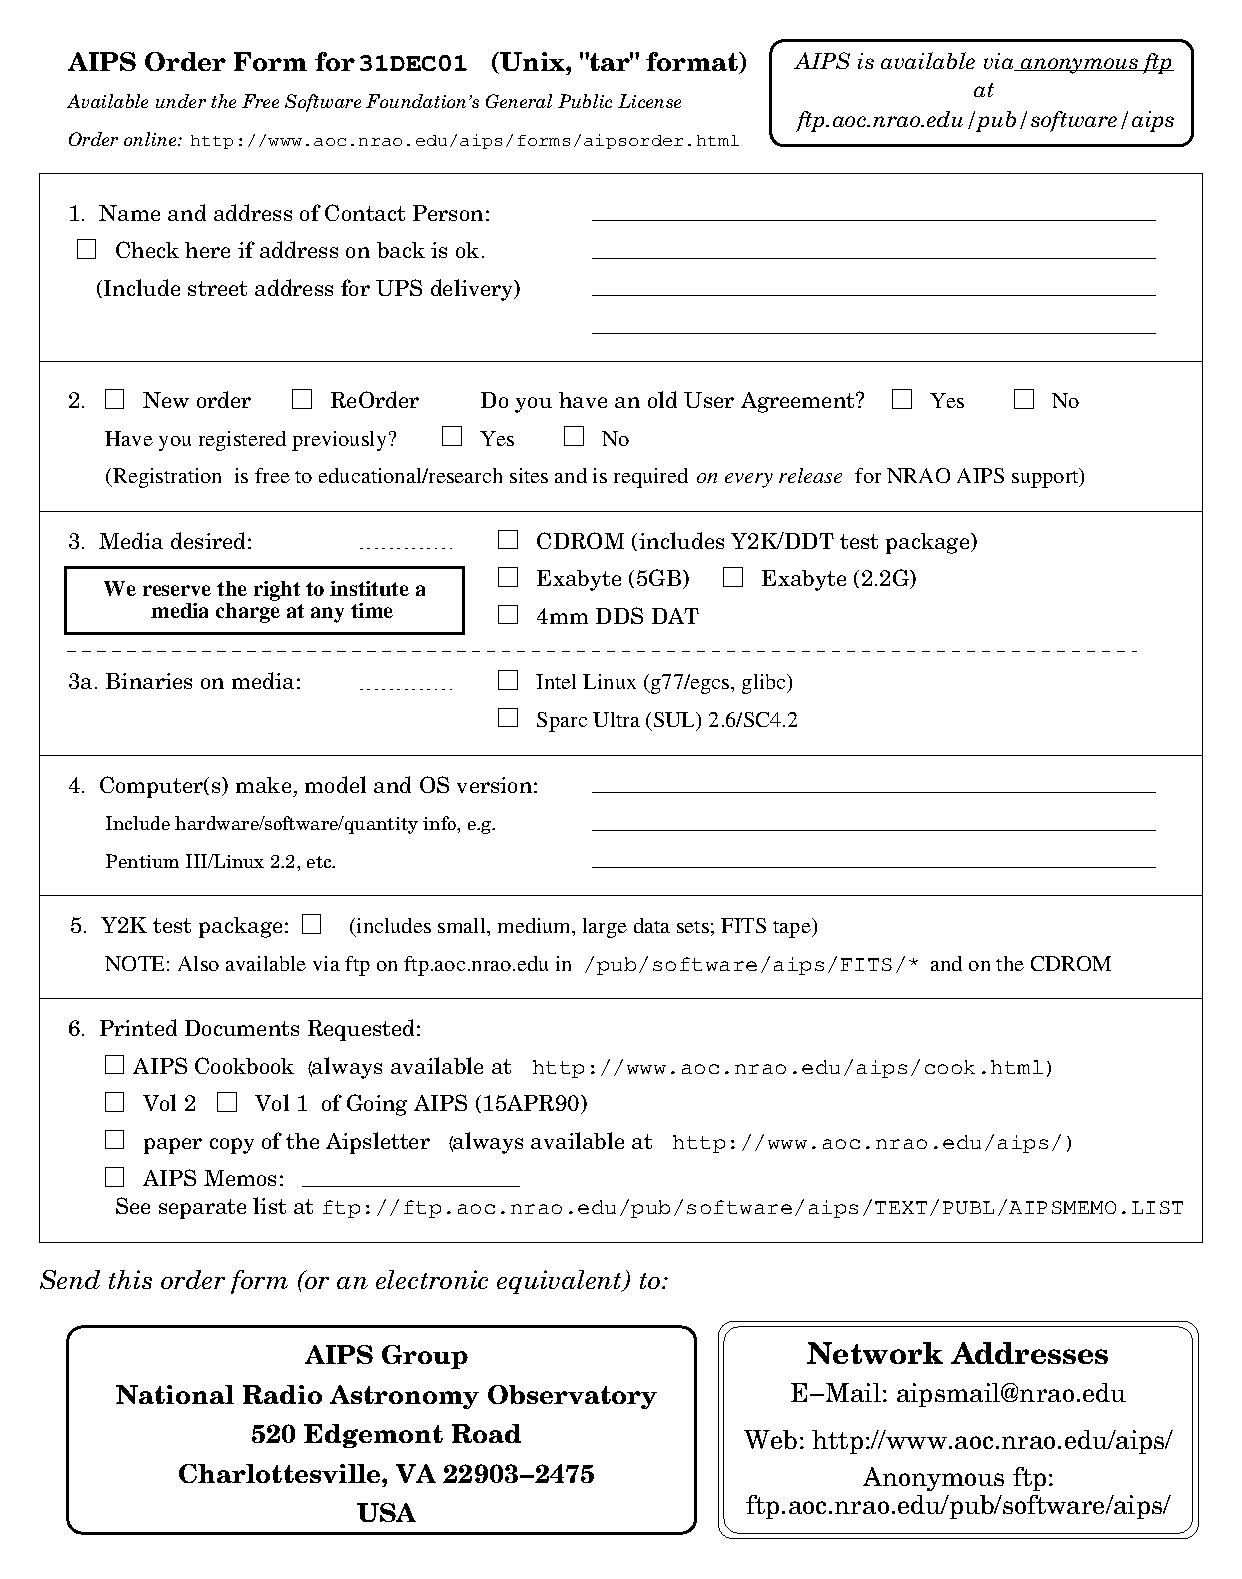
\includegraphics{FIG/AIPSORDER.PS}}}
\vfill\eject
 \vbox to 4.4in{
  \vspace{12pt}
%  \vfill
%  \centerline{\resizebox{!}{2.6in}{\includegraphics{FIG/Mandrill.eps}}}
  \centerline{\rotatebox{-90}{\resizebox{!}{3.5in}{%
\includegraphics{FIG/KNTR3.plt}}}}
  \vspace{12pt}
  \centerline{{\huge \tt \AIPRELEASE}}
  \vspace{12pt}
  \vfill}
\phantom{...}
\centerline{\resizebox{!}{!}{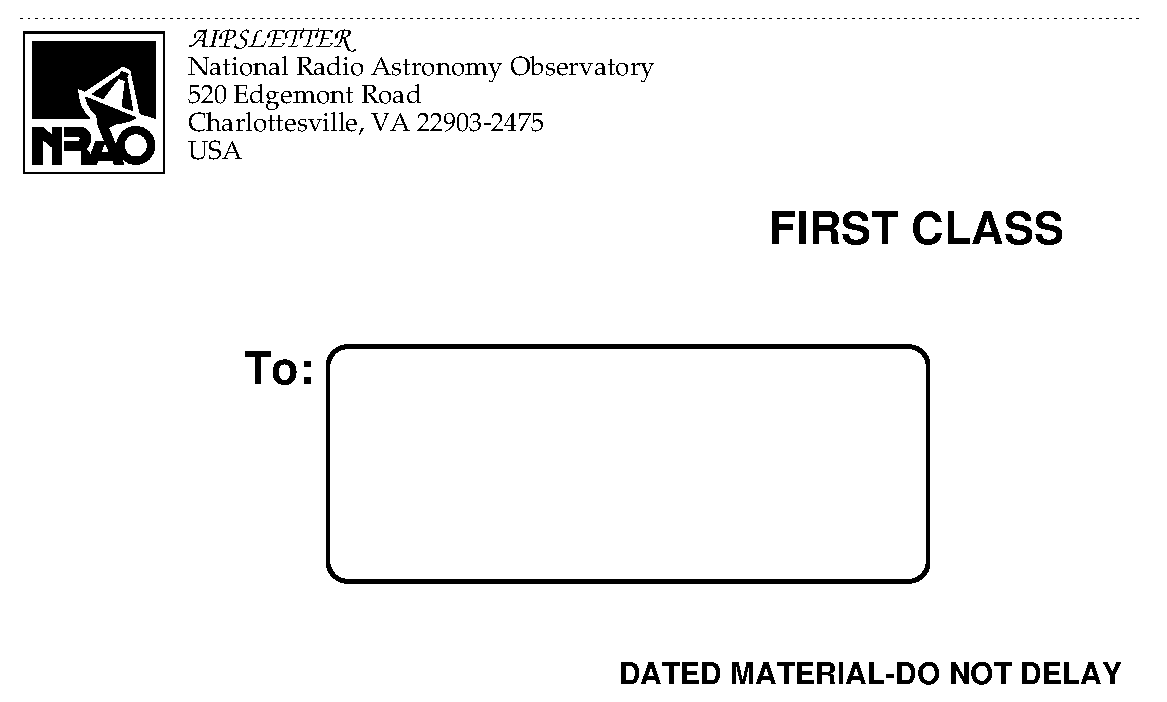
\includegraphics{FIG/AIPSLETM.PS}}}

\end{document}
